\vspace{1em}
\begin{minipage}[t]{11cm}
  \vspace{-1.7cm}
  \section{Signal Modeling \hayes{129}}
  %\renewcommand{\arraystretch}{1.0}
  \textbf{Objective: } Calculate the coefficients for a filter whose
  impulse response matches as closely as possible with a given signal ($x[n]$ - with
  length $N$).

      $$ y(n) = \sum\limits_{k=0}^{q} b(k)x(n-k) - \sum\limits_{k=1}^{p} a(k)y(n-k)$$
      $$ H(z) = \dfrac{B(z)}{A(z)} = \dfrac{b_0 + b_1z^{-1} + b_2 z^{-2} + \dots +
      b_q z^{-q}}{1 + a_1z^{-1} + a_2 z^{-2} + \dots + a_p z^{-p}} $$

\end{minipage}
\hfill
\begin{minipage}{7.2cm}
	\vspace{3mm}
	\begin{tabular}{| p{1.4cm} | p{2cm} | p{2.2cm} | }
	    \hline
	    \textbf{Method}
	    & exact match
	    & minimal error \\
	    \hline
	    \hline
	    \textbf{LS}
	    & $[0]$
	    & $[1, N - 1]$\\
	    \hline
	    \textbf{Padé}
	    & $[0, q + p + 1]$
	    & -\\
	    \hline
	    \textbf{Prony}
	    & $[0, q]$
	    & $[q + 1, N - 1]$ \\
	    \hline
	    \textbf{Shanks}
	    & $[0]$
	    & $[1, N - 1]$\\
	    \hline
	\end{tabular}\\
	$q$: number of zeros\\
	$p$: number of poles\\
	$N$: length of signal $x(n)$
\end{minipage}

\subsection{Least Squares Method \hayes{131}}
The coefficients \textbf{A and B} are estimated using the least squares error method.
Since solving the estimation requires a $p+q$ equation system, this method is very rarely applied.\\
\begin{minipage}{8cm}
	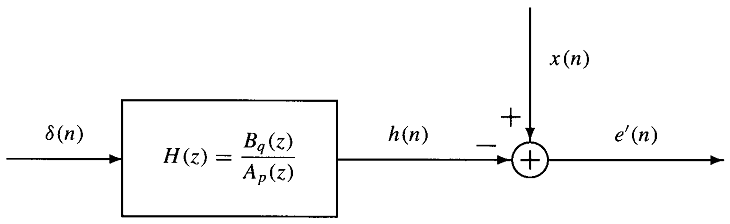
\includegraphics[width=8cm]{../TSM_StatDig/bilder/signalModeling.png}
\end{minipage}
\begin{minipage}{10cm}
$\frac{\partial \sum\limits_{n=0}^{\infty}|e'(n)|^2}{\partial a_p^*(k)}=\frac{1}{2\pi} \int\limits_{-\pi}^{\pi}\left[X(e^{j\omega})-
\frac{B_q(e^{j\omega})}{A_p (e^{j\omega})}\right]\frac{B^*_q(e^{j\omega})}{A_p^* (e^{j\omega})^2}e^{jk\omega} d\omega=0$\\
$\frac{\partial \sum\limits_{n=0}^{\infty}|e'(n)|^2}{\partial b_q^*(k)}=\frac{1}{2\pi} \int\limits_{-\pi}^{\pi}\left[X(e^{j\omega})-
\frac{B_q(e^{j\omega})}{A_p (e^{j\omega})}\right]\frac{e^{jk\omega}}{A_p^* (e^{j\omega})} d\omega=0$\\
\end{minipage}
\subsubsection{Example FIR Equalizer}
With a FIR first order (2 coefficients) a given sequence (e.g. $[0, 2, 1, 0]$ ) should be filtered so that output is a Dirac $[0, 1 , 0 , 0]$.\\
$\underbrace{\begin{bmatrix}
x[0] 	& 0 	\\
x[1]	& x[0]	\\
0		& x[1]
\end{bmatrix}}_{\bm A}
\cdot \begin{bmatrix}
b_0\\
b_1
\end{bmatrix}=\begin{bmatrix}
1\\
0\\
0
\end{bmatrix}$. To solve the equations the pseudo inverse has to be used: $\bm A^{\dagger} = \left(\bm A^T \cdot \bm A\right)^{-1}\bm A^T
\Rightarrow \bm  A^\dagger \begin{bmatrix}
1\\
0\\
0
\end{bmatrix}=\begin{bmatrix}
b_0\\
b_1
\end{bmatrix}$

\subsection{Padé Approximation}
The resulting impulse response \textbf{matches exactly} with the given signal $x[n]$ in the interval $[0, q + p + 1]$,
afterwards, the filter is not necessarily stable.

	%\vspace{-0.5cm}
	\renewcommand{\arraystretch}{1.0}
	\begin{aufzaehlung}
  		\item Calculate $a$-coefficients / poles: $\bm X_q \cdot a_p = -x_{q+1} \Longrightarrow a_p = - \bm X_q^{-1} \cdot x_{q+1}$ \small $$
	%	\begin{matrix} n=q+1\\ n=q+2\\ \vdots \\ n=q+p \end{matrix}
		\underbrace{ \begin{bmatrix}
    		x[q]     & x[q-1]   & \hdots & x[q-p+1] \\
    		x[q+1]   & x[q]     & \hdots & x[q-p+2] \\
    		\vdots   & \vdots   & \ddots & \vdots \\
    		x[q+p-1] & x[q+p-2] & \hdots & x[q] \\
		\end{bmatrix}
		}_{\bm  X_q} \cdot
		\underbrace{\begin{bmatrix}
    		a_1 \\
    		a_2 \\
    		\vdots \\
    		a_p
		\end{bmatrix}  }_{a_p} = \underbrace{\begin{bmatrix}
    		-x [q+1]\\
    		-x [q+2]\\
    		\vdots \\
    		-x [q+p]\\
		\end{bmatrix}}_{x_{q+1}}  \Longleftrightarrow
		\begin{bmatrix}
    		x[q+1] & x[q] & \hdots & x[q+1-p] \\
    		x[q+2] & x[q+1] & \hdots & x[q+2-p] \\
    		\vdots & \vdots & \ddots & \vdots \\
    		x[q+p] & x[q+p-1] & \hdots & x[q] \\
		\end{bmatrix}
		\begin{bmatrix}
    		1 \\
    		a_1 \\
    		\vdots \\
    		a_p
		\end{bmatrix} =
		\begin{bmatrix}
    		0 \\
    		0 \\
    		\vdots \\
    		0
		\end{bmatrix}
		$$  \normalsize

		\vspace{-0.5cm}
		If \(\bm X_q\) is singular, the assumption that $a_0 = 1$ was incorrect. $\Longrightarrow$ Set $a_0=0$.
		$ \Longrightarrow \bm X_q \cdot \bm a_p = \bm 0$

  		\item Calculate $b$-coefficients / zeros: $\bm X_0 \cdot a_p = b_q$ \small \hspace{0.5cm}
		$ \begin{matrix} n=0\\ n=1\\ \vdots\\ n=q \end{matrix} \overset{(0 \hdots p)}{\underbrace{\begin{bmatrix}
    		x[0] & 0 & \hdots & 0 \\
    		x[1] & x[0] & \hdots & 0 \\
    		\vdots & \vdots & \ddots & \vdots \\
    		x[q] & x[q-1] & \hdots & x[q-p]
		\end{bmatrix}  }_{\bm X_0}}\cdot \underbrace{\begin{bmatrix}
    		1 \\
    		a_1 \\
    		\vdots \\
    		a_p
		\end{bmatrix}  }_{a_p}= 	\underbrace{\begin{bmatrix}
	    		b_0 \\
	    		b_1 \\
	    		\vdots \\
	    		b_q
			\end{bmatrix}}_{b_q}$ \normalsize

	\end{aufzaehlung}

\vspace{-1.0cm}


\subsection{Prony's Method \hayes{144}}
The resulting impulse response \textbf{matches exactly} with the given signal $x[n]$ in the interval $[0, q]$.
In the interval $[q + 1, N-1]$, the values are approximated with the
\textbf{least squares error} (overdetermined system of equations).


\renewcommand{\arraystretch}{1.0}

\begin{aufzaehlung}
	\item Calculate autocorrelation: $ r_x(k,l) = \sum\limits_{n=q+1}^\infty x(n-l)x^*(n-k)$;\qquad $k,l\geq 0$
	\item Calculate $a$-coefficients: $\bm R_x \cdot a_p = -r_x \Longrightarrow a_p = - \bm R_x^{-1} \cdot r_x$
  		\small\\
		The minimal error is: $\epsilon_{p,q} = r_x(0,0) + \sum\limits_{k=1}^p a_p(k) r_x(0,k)$
			$$
		\underbrace{\begin{bmatrix}
    		r_x[1,1] & r_x[1,2] & \hdots & r_x[1,p] \\
    		r_x[2,1] & r_x[2,2] & \hdots & r_x[2,p] \\
    		\vdots & \vdots & \ddots & \vdots \\
    		r_x[p,1] & r_x[p,2] & \hdots & r_x[p,p] \\
		\end{bmatrix}  }_{\bm R_x} \cdot
		\underbrace{\begin{bmatrix}
    		a_1 \\
    		\vdots \\
    		a_p
		\end{bmatrix}  }_{a_p}= -\underbrace{\begin{bmatrix}
    		r_x[1,0] \\
    		\vdots \\
    		r_x[p,0]
		\end{bmatrix}  }_{r_x}
		\Longrightarrow
		\begin{bmatrix}
    		r_x[0,0] & r_x[0,1] & \hdots & r_x[0,p] \\
    		----&----&----&----\\
    		r_x[1,0] & r_x[1,1] & \hdots & r_x[1,p] \\
    		r_x[2,0] & r_x[2,1] & \hdots & r_x[2,p] \\
    		\vdots & \vdots & \ddots & \vdots \\
    		r_x[p,0] & r_x[p,1] & \hdots & r_x[p,p] \\
		\end{bmatrix} \cdot
		\begin{bmatrix}
    		1 \\
    		a_1 \\
    		\vdots \\
    		a_p
		\end{bmatrix} = \begin{bmatrix}
    		\epsilon_{p,q} \\
    		---\\
    		0 \\
    		\vdots \\
    		0
		\end{bmatrix} $$
		For all-pole models, the a-coefficients can be directly calculated from the b system of equations.
		For this, all $b$-coefficients except for $b_0$ must be set to 0.
	\item Calculate $b$-coefficients as in \textbf{Padé}: $\bm X_0 \cdot a_p = b_q$
		\normalsize
\end{aufzaehlung}

\subsection{Shanks' Method \hayes{154}}

The B-coefficients are estimated given the A's in such a way that the resulting impulse response in the interval $[0, N - 1]$ with the
\textbf{least squares error} (overdetermined system of equations) approximates the given
signal $x[n]$. The only improvement would be if the A-coefficients could also include all signal values (Least-square).

\begin{aufzaehlung}
  		\item Calculate $a$-coefficients as in \textbf{Prony}: $a_p = - \bm R_x^{-1} \cdot r_x$
  		\item Calculate impulse response $g[n]$ of the purely recursive filter ($g[n] = \delta(n)- \sum\limits_{k=1}^p a_p(k)g(n-k)$),
  		or using inverse z-transform of $H(z)$.
  		\item Calculate autocorrelation:  $r_g(k)=\sum\limits_{n=0}^\infty g(n)g^*(n-k)$; or inverse z-transform of $|H(z)|^2$
  		\item Calculate cross-correlation: $r_{xg}(k)=\sum\limits_{n=0}^\infty x(n)g^*(n-k)$
  		\item Calculate $b$-coefficients (for stationary processes): $b_q = R_g^{-1} \cdot r_{xg}$ \\
  		for\\

		 $$\begin{matrix}n=0\\ n=1\\ \vdots\\ n=N_{ha}+q\\ \end{matrix}
		\overset{(0 \hdots q)}{\underbrace{\begin{bmatrix}
    		r_g(0) & r_g(1) & \hdots & r_g(q) \\
    		r_g(1) & r_g(0) & \hdots & r_g(q-1) \\
    		\vdots & \vdots & \ddots & \vdots \\
    		r_g(q) &r_g(q-1) & \hdots & r_g(0) \\
		\end{bmatrix}  }_{R_g}} \cdot \underbrace{\begin{bmatrix}
    		b_0 \\
    		b_1 \\
    		\vdots \\
    		b_q
		\end{bmatrix}  }_{b_q}= \underbrace{\begin{bmatrix}
    		r_{xg}(0) \\
    		r_{xg}(1) \\
    		\vdots \\
    		r_{xg}(q) \\
		\end{bmatrix}  }_{r_{xg}} $$
\end{aufzaehlung}

\subsection{All-Pole Modeling \hayes{160}}
Corresponds to: \ref{sec:autoregressive_model_method}
\begin{enumerate}
	\item Calculate autocorrelation: $ r_x(k) = \sum\limits_{n=0}^\infty x(n)x^*(n-k)$;\qquad $k\geq 0$
	\item Calculate $a$-coefficients: $\bm R_x \cdot a_p = -r_x \Longrightarrow a_p = - \bm R_x^{-1} \cdot r_x$
  		\small\\
		The minimal error is: $\epsilon_{p} = r_x(0) + \sum\limits_{k=1}^p a_p(k) r_x^*(k)$
			$$
		\underbrace{\begin{bmatrix}
    		r_x(0) & r_x^*(1) & \hdots & r_x^*(p-1) \\
    		r_x(1) & r_x(0) & \hdots & r_x^*(p-2) \\
    		\vdots & \vdots & \ddots & \vdots \\
    		r_x(p-1) & r_x(p-2) & \hdots & r_x(0) \\
		\end{bmatrix}  }_{\bm R_x} \cdot
		\underbrace{\begin{bmatrix}
    		a_1 \\
    		\vdots \\
    		a_p
		\end{bmatrix}  }_{a_p}= -\underbrace{\begin{bmatrix}
    		r_x(1) \\
    		\vdots \\
    		r_x(p)
		\end{bmatrix}  }_{r_x}$$
	\item $b(0) = \sqrt{\epsilon_p}$
\end{enumerate}


\subsection{Linear Prediction \hayes{165} (Exercise 4.13)}

		$$\hat{x}(n+n_0) = - \sum\limits_{k=1}^p a_p(k) x(n-k)$$
		$$
		\underbrace{\begin{bmatrix}
    		r_x[1,1] & r_x[1,2] & \hdots & r_x[1,p] \\
    		r_x[2,1] & r_x[2,2] & \hdots & r_x[2,p] \\
    		\vdots & \vdots & \ddots & \vdots \\
    		r_x[p,1] & r_x[p,2] & \hdots & r_x[p,p] \\
		\end{bmatrix}  }_{\bm R_x} \cdot
		\underbrace{\begin{bmatrix}
    		a_1 \\
    		\vdots \\
    		a_p
		\end{bmatrix}  }_{a_p}= \underbrace{\begin{bmatrix}
    		r_x[1,-n_0] \\
    		\vdots \\
    		r_x[p,-n_0]
		\end{bmatrix}  }_{r_x}$$

\subsection{FIR Inverse Filter \hayes{166}}
$$G(z)H(z) \approx 1\qquad g(n)*h(n) \approx \delta(n) \qquad r_g(k) = \sum\limits_{n=0}^\infty g(n)g^*(n-k) \qquad \text{Delay: } n_0$$

		$$
		\underbrace{\begin{bmatrix}
    		r_g(0) & r_g(1) & \hdots & r_g(N-1) \\
    		r_g(1) & r_g(0) & \hdots & r_g(N-2) \\
    		\vdots & \vdots & \ddots & \vdots \\
    		r_g(N-1) & r_g(N-2) & \hdots & r_g(0) \\
		\end{bmatrix}  }_{\bm R_g} \cdot
		\underbrace{\begin{bmatrix}
    		h_N(0) \\
    		\vdots \\
    		h_N(N-1)
		\end{bmatrix}  }_{h_N}= -\underbrace{\begin{bmatrix}
    		g(n_0) \\
    		g(n_0 - 1)	 \\
    		\vdots \\
    		g(0)\\
    		0\\
    		\vdots \\
    		0
		\end{bmatrix}  }_{r_{gd}}$$


		\subsection{Approximation with limited data using All-Pole Filter}
		\subsubsection{Autocorrelation Method \hayes{178}}
		Given the autocorrelations, see Chapter \ref{sec:autoregressive_model_method}.\\
		Assumption: The data $x[n]$ is zero outside the definition range $[0,N]$. This forces the filter into a stable state.
		\renewcommand{\arraystretch}{1.0}

		\begin{enumerate}
			\item Calculate $a$-coefficients (using Pseudoinverse / generalized Inverse): $a_p = -\left(\bm X_p^T \cdot \bm  X_p\right)^{-1} \cdot \bm X_p^T \cdot x_1$
				\small
				$$
				\begin{matrix} n=q+1\\ n=q+2\\ \vdots \\ n=N\\ n=N+1\\ \vdots \\ N+p
				\end{matrix}
				\underbrace{\begin{bmatrix}
					x[0] & 0 & \hdots & 0 \\
					x[1] & x[0] & \hdots & 0 \\
					x[2] & x[1] & \hdots & 0 \\
					\vdots & \vdots & \ddots & \vdots \\
					----&----&----&----\\
					x[p-1] & x[p-2] & \hdots & x[0] \\
					x[p] & x[p-1] & \hdots & x[1] \\
					\vdots & \vdots & \ddots & \vdots \\
					x[N-1] & x[N-2] & \hdots & x[N-p] \\
					----&----&----&----\\
					x[N] & x[N-1] & \hdots & x[N-p+1] \\
					0 & x[N] & \hdots & x[N+2-p] \\
					\vdots & \vdots & \ddots & \vdots \\
					0 & 0 & \hdots & x[N] \\
				\end{bmatrix}  }_{\bm X_p=(N+p \; \times \; p)\text{-Matrix}} \cdot \underbrace{\begin{bmatrix}
					a_1 \\
					\vdots \\
					a_p
				\end{bmatrix}  }_{a_p}= \underbrace{\begin{bmatrix}
					 -x [1]\\
					 -x [2]\\
					\vdots \\
					 -x [N]\\
					0 \\
					\vdots \\
					0
				\end{bmatrix}}_{x_1}
				 $$ \normalsize
			\end{enumerate}

		\subsubsection{Covariance Method  \hayes{183}}
		No assumptions are made, only the existing data is used. A disadvantage is that the filter can become unstable.
		Another disadvantage is that \(\bm X\) is not a Toeplitz matrix, so solving it is not as straightforward as with the Autocorrelation Method.
		However, the signal is reconstructed more accurately.
		For a data series corresponding to an impulse response, the filter is perfectly reconstructed (as long as \(N \ge 2p\)).
		With the disadvantage that unstable poles are also implemented.
		\begin{minipage}{0.7\linewidth}
			\small
			$$
			\underbrace{\begin{bmatrix}
				x[p-1] & x[p-2] & \hdots & x[0] \\
				x[p] & x[p-1] & \hdots & x[1] \\
				\vdots & \vdots & \ddots & \vdots \\
				x[N-1] & x[N-2] & \hdots & x[N-p] \\
			\end{bmatrix}  }_{\bm X_p=(N-p+1 \; \times \; p)\text{-Matrix}} \cdot \underbrace{\begin{bmatrix}
				a_1 \\
				\vdots \\
				a_p
			\end{bmatrix}  }_{a_p}= \underbrace{\begin{bmatrix}
					-x[p]\\
					-x[p+1]\\
				\vdots \\
					-x[N]\\
			\end{bmatrix}}_{x_p}
			$$ \normalsize
		\end{minipage}
		\begin{minipage}[t]{0.3\linewidth}
			$a_p = -\left(\bm X_p^T \cdot \bm  X_p\right)^{-1} \cdot \bm X_p^T \cdot x_p$
		\end{minipage}
		(Note: These equations are a subset of the equations of the Autocorrelation Method.)


\subsection{Stochastic Models}
In stochastic models, generally the same models are used as in the deterministic world.
Instead of the Dirac pulse, white noise is used at the input of the filter, and the autocorrelation is formed using the expected value.
$r_x(k)=E\{x(n) \cdot x^*(n-k)\}$\\
Instead of the cross-correlation $r_{gx}$, the convolution of $b_q(k)$ and $h^*(-k)$ is used.\\
$c_q(k) = b_q(k) \ast h^*(-k) = \sum_{l=0}^{q-k} b_q(l+k) h^*(l)$

\subsubsection{Autoregressive Moving Average Models, ARMA \hayes{189}}
An ARMA(p,q) process is white noise that is filtered through an LTI system $H(z)$.\\
To determine the coefficients of $H(z)=\frac{B_q(z)}{A_p(z)}=\frac{\sum\limits_{k=0}^q b_q(k)z^{-k}}{1+\sum\limits_{k=1}^p a_p(k)z^{-k}}$, the \textbf{extended Yule-Walker equations} are solved:
\small$$
\underbrace{\begin{bmatrix}
			r_x[0] & r_x^*[1] & \hdots & r_x^*[p] \\
			r_x[1] & r_x[0] & \hdots & r_x^*[p-1] \\
			\vdots & \vdots & \ddots & \vdots \\
			r_x[q] & r_x[q-1] & \hdots & r_x[q-p] \\
			r_x[q+1] & r_x[q] & \hdots & r_x[q-p+1] \\
			\vdots & \vdots & \ddots & \vdots \\
			r_x[L] & r_x[L-1] & \hdots & r_x[L-p] \\
		\end{bmatrix}  }_{R_x} \cdot \underbrace{\begin{bmatrix}
			1\\
			a_p(1) \\
			a_p(2) \\
			\vdots \\
			a_p(p)
		\end{bmatrix}  }_{a_p}= \begin{bmatrix}
				c_q[0]\\
				c_q[1]\\
			\vdots \\
				c_q[q]\\
				0\\
			\vdots \\
				0\\
		\end{bmatrix}
			$$ \normalsize

\begin{aufzaehlung}
			\item Calculate the A- coefficients: $R_q \cdot a_p = - r_{q+1}$
			\small$$
\underbrace{\begin{bmatrix}
			r_x[q] & r_x[q-1] & \hdots & r_x[q-p+1] \\
			r_x[q+1] & r_x[q] & \hdots & r_x[q-p+2] \\
			\vdots & \vdots & \ddots & \vdots \\
			r_x[q+p-1] & r_x[q+p-2] & \hdots & r_x[q] \\
		\end{bmatrix}  }_{R_q} \cdot \underbrace{\begin{bmatrix}
			a_p(1) \\
			a_p(2) \\
			\vdots \\
			a_p(p)
		\end{bmatrix}  }_{a_p}= \underbrace{\begin{bmatrix}
				-r_x[q+1]\\
				-r_x[q+2]\\
			\vdots \\
				-r_x[q+p]\\
		\end{bmatrix}}_{r_{q+1}}
			$$ \normalsize
			\item To calculate the B- coefficients, one must go via the C- coefficients: $R_x \cdot a_p = c_q$

			\small$$
\underbrace{\begin{bmatrix}
			r_x[0] & r_x^*[1] & \hdots & r_x^*[p] \\
			r_x[1] & r_x[0] & \hdots & r_x^*[p-1] \\
			\vdots & \vdots & \ddots & \vdots \\
			r_x[q] & r_x[q+1] & \hdots & r_x[0] \\
		\end{bmatrix}  }_{R_x} \cdot \underbrace{\begin{bmatrix}
			1 \\
			a_p(1) \\
			a_p(2) \\
			\vdots \\
			a_p(p)
		\end{bmatrix}  }_{a_p}= \underbrace{\begin{bmatrix}
				c_q[0]\\
				c_q[1]\\
			\vdots \\
				c_q[q]\\
		\end{bmatrix}}_{c_{q}}
			$$ \normalsize
			\item Write down $[C_q(z)]_+$: $[C_q(z)]_+ = \sum\limits_{k=0}^q c_q(k)z^{-k}$
			\item Calculate $[P_y(z)]_+=\left[[C_q(z)]_+ \cdot A^*_p(1/z^*)\right]_+$ e.g. $[C_1(z)]_+=\frac{45}{2}-6z^{-1}$, $A^*_p(1/z^*)=1-0.5z$; $[C_1(z)]_+ \cdot A^*_p(1/z^*)= -\frac{45}{4}z +\frac{51}{2}-6z^{-1}$ $\Rightarrow$  $[P_y(z)]_+= \frac{51}{2}-6z^{-1}$
			\item Make $[P_y(z)]_+$ symmetric. e.g.: $P_y(z) =  -6 z +\frac{51}{2}-6z^{-1}$
			\item Factorize $P_y(z)=B_q(z)B_q^*(1/z^*)$ so $B_q(z)$ can be used: \\
			e.g. $B_1(z)\cdot B_1^*(1/z^*)= \underbrace{2\sqrt{6}(1-\frac{1}{4}z^{-1})}_{B_q(z)}\cdot \underbrace{2\sqrt{6}(1-\frac{1}{4}z^{1})}_{B_q^*(1/z^*)}$
			\item $H(z)=\frac{B_q(z)}{A_p(z)}$ e.g.: $H(z)=\frac{2 \sqrt{6}(1-\frac 1 4 z^{-1})}{A_p(z)}$
\end{aufzaehlung}


\subsubsection{Autoregressive Models - AR \hayes{194}}
\label{sec:autoregressive_model_method}
In the AR(p) model, the ARMA(p,q=0) method is used, but only with poles. $H(z)=\frac{b(0)}{1+\sum\limits_{k=1}^{p} a_p(k)z^{-k}}$.\\
 $$\begin{bmatrix}
	 	r_x(0)  & r_x^*(1) & r_x^*(2) & \cdots & r_x^*(p-1)\\
	 	r_x(1)  & r_x(0) & r_x^*(1) & \cdots & r_x^*(p-2)\\
	 	r_x(2)  & r_x(1) & r_x(0) & \cdots & r_x^*(p-3)\\
	 	\vdots  & \vdots  & \vdots  & \ddots & \vdots\\
	 	r_x(p-1)& r_x(p-2)& r_x(p-3)& \cdots &  r_x(0)\\
   \end{bmatrix} \cdot
   \begin{bmatrix}
    	a_p(1)\\
    	a_p(2)\\
    	a_p(3)\\
    	\vdots\\
    	a_p(p)\\
   \end{bmatrix}=
   \begin{bmatrix}
       	-r_x(1)\\
       	-r_x(2)\\
       	-r_x(3)\\
       	\vdots\\
        -r_x(p)\\
   \end{bmatrix}
 $$
 With $|b(0)|^2=r_x(0) + \sum\limits_{k=1}^{p} a_p(k)r_x(k)$



 \subsubsection{Moving Average Models - MA \hayes{195}}
A MA process is a special form of an ARMA(p=0,q) process, which only has zeros.\\
$P_x(z)=\sum\limits_{k=-q}^{q}r_x(k)z^{-k}=B_q(z)B_q^*(1/z^*)$
\begin{aufzaehlung}
	\item Spectrally factorize $P_x(z)$ into: $P_x(z)=\sigma^2_0 \cdot Q(z)\cdot Q^*(1/z^*)=\underbrace{\sigma^2_0}_{|b_q(0)|^2} \underbrace{\prod\limits_{k=1}^q (1-\beta_k z^{-1})}_{B_q(z)} \cdot \underbrace{\prod\limits_{k=1}^q (1-\beta_k^* z)}_{B^*_q(1/z^*)}$
	\item Expand $B_q(z)$ $\Rightarrow$ minimum phase filter (all zeros are inside the unit circle)
	\item Or, expand $B_q^*(1/z^*)$ to get a maximum phase filter (all zeros are outside the unit circle)
\end{aufzaehlung}
